\documentclass[cjk,slidestop,compress,mathserif,blue]{beamer}
%dvipdfm选项是关键,否则编译统统通不过
%beamer的颜色选项定义的是导航条和标题的颜色(即关键词structure的颜色)

%%%%%%%%%%%%%%%%仅限于XeTeX可使用的宏包%%%%%%%%%%%%%%%%%%%%%%%%%%%%
\usepackage{fontspec,xunicode,xltxtra,beamerthemesplit}
%\usepackage{beamerthemesplit}
\usepackage{xeCJK}
\setCJKmainfont[BoldFont=黑体, ItalicFont=楷体, BoldItalicFont=仿宋]{黑体}
%\setsansfont[Mapping=tex-text]{Adobe 黑体 Std}
%如果装了Adobe Acrobat,可在font.conf中配置Adobe字体的路径以使用其中文字体
%也可直接使用系统中的中文字体如SimSun,SimHei,微软雅黑 等
%原来beamer用的字体是sans family;注意Mapping的大小写,不能写错

%%%%%%%%   确定标题和导航条结构的框架     %%%%%%%%%%%%
\usepackage{beamerthemeshadow}                       %
%\usepackage{beamerthemeclassic}%导航条色与背景色一致%
%%%%%%%%%%%%%%%%%%%%%%%%%%%%%%%%%%%%%%%%%%%%%%%%%%%%%%
\setbeamerfont{roman title}{size={}}
%\usepackage{CJK} % CJK 中文支持                                  %
\usepackage{amsmath,amsthm,amsfonts,amssymb,bm}
\usepackage{mathrsfs}
\usepackage{xcolor}                                        %使用默认允许使用颜色
\usepackage{hyperref} 
\usepackage{graphicx}
\usepackage{subfigure}           %图片跨页

%\usepackage[numbers,sort&compress]{natbib} %紧密排列             %
\usepackage[sectionbib]{chapterbib}        %每章节单独参考文献   %
\usepackage{hypernat}                                                                         %
%\usepackage[dvipdfm,bookmarksopen=true,pdfstartview=FitH,CJKbookmarks]{hyperref}		%
\hypersetup{bookmarksnumbered,colorlinks,linkcolor=brown,citecolor=blue,urlcolor=red}         %
%参考文献含有超链接引用时需要下列宏包,注意与natbib有冲突        %
%\usepackage[dvipdfm]{hyperref}                                  %
%\usepackage{hypernat}                                           %
\newcommand{\upcite}[1]{\hspace{0ex}\textsuperscript{\cite{#1}}} %

%\useoutertheme{smoothbars}
\useinnertheme[shadow=true]{rounded}
\usetheme{Berkeley}                                          %主题式样
%\usetheme{Luebeck}

\usecolortheme{lily}                                        %颜色主题式样

\usefonttheme{professionalfonts}                           %字体主题样式宏包

%\beamertemplatetransparentcoveredhigh                      %使所有被隐藏的文本高度透明
\beamertemplatetransparentcovereddynamicmedium             %使所有被隐藏的文本完全透明,动态,动态的范围很小
\mode<presentation>
%\beamersetaveragebackground{gray}                          %设置背景颜色(单一色) 
\beamertemplateshadingbackground{green!10}{red!5}         %设置背景颜色(渐变色)


\begin{document}
%\begin{CJK*}{GBK}{song}
%\begin{CJK*}{GBK}{kai}
%beamer下不能用\songyi、\zihao等命令!
%\graphicspath{Figures/}

%-------------------------------PPT Title-------------------------------------
\title{PAW方法概述}
%-----------------------------------------------------------------------------

%----------------------------Author & Date------------------------------------
\author{北京市计算中心\;云平台\:姜骏}
\date{\textrm{2016.09.30}}
%\date{2013.09.10}
\frame{\titlepage}
%-----------------------------------------------------------------------------

%------------------------------------------------------------------------------列出全文 outline ---------------------------------------------------------------------------------
\section*{}
\frame[allowframebreaks]
{
  \frametitle{Outline}
%  \frametitle{\textcolor{mycolor}{\secname}}
  \tableofcontents%[current,currentsection,currentsubsection]
}
%在每个section之前列出全部Outline
%类似的在每个subsection之前列出全部Outline是\AtBeginSubsection[]
\AtBeginSection[]
{
  \frame<handout:0>
  {
    \frametitle{Outline}
%全部Outline中,本部分加亮
    \tableofcontents[current,currentsection]
  }
}

%------------------------------------------------------------------------------PPT main Body------------------------------------------------------------------------------------
\small
%\section{Induction on DFT and solid-state physics}       %Bookmark
\frame
{
	\frametitle{赝势方法发展概要}
\begin{figure}[h!]
\centering
\vspace*{-0.25in}
%\hspace*{-0.80in}
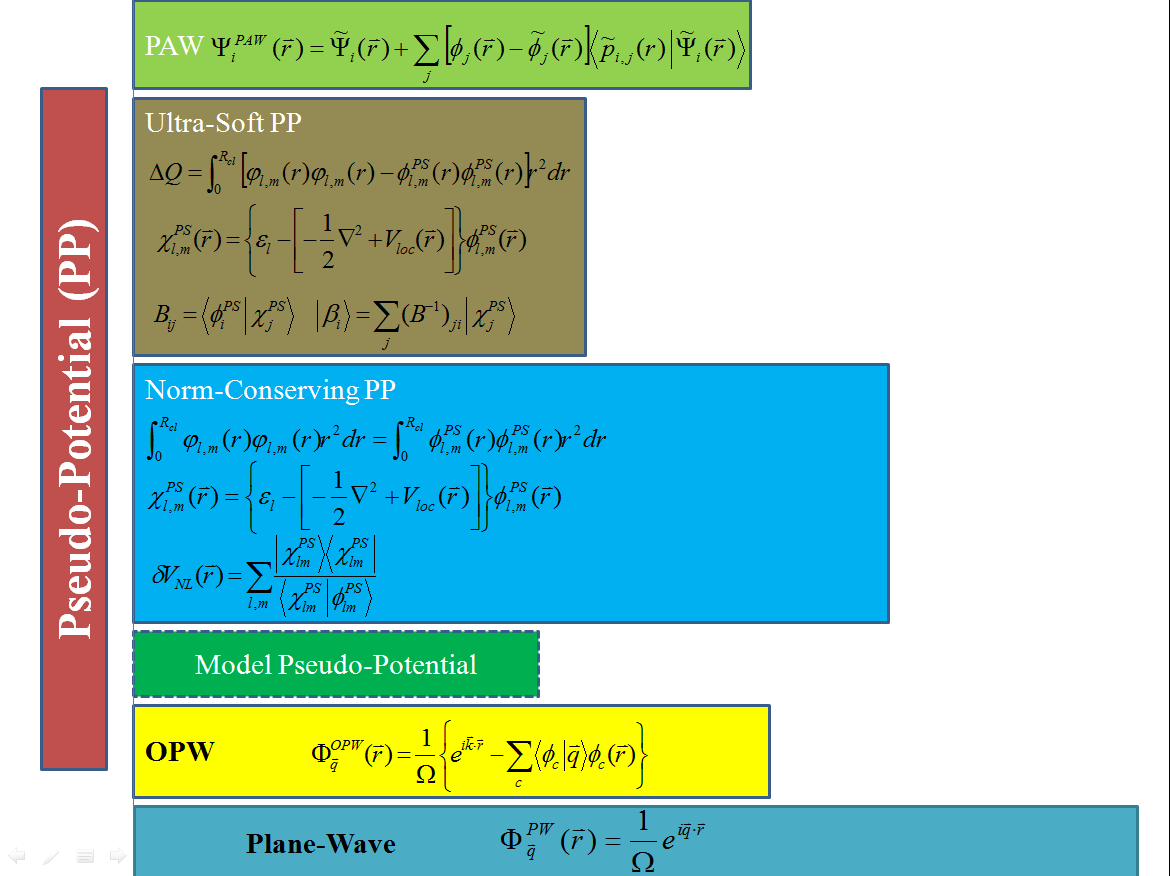
\includegraphics[height=2.80in,width=4.10in,viewport=0 0 1190 875,clip]{Figures/Pseudo_Potential.png}
%\caption{\small \textrm{Pseudopotential for metallic sodium, based on the empty core model and screened by the Thomas-Fermi dielectric function.}}%(与文献\cite{EPJB33-47_2003}图1对比)
\label{Pseudo_Poential}
\end{figure}
}

\section{$\mathrm{PAW}$方法概要}
\frame
{
	\frametitle{\textrm{PAW}方法概要}
\begin{itemize}
	\item 与芯层态正交的全部价电子构成的\textrm{Hilbert}空间%,价电子彼此的正交使得波函数在\textrm{Muffin-tin}球内振荡
	\item 作\textcolor{red}{线性空间变换},全电子波函数$|\Psi\rangle$与赝波函数$|\tilde\Psi\rangle$满足:
		$$|\Psi\rangle=\mathbf{\tau|}\tilde\Psi\rangle$$
%	$$\tau=\mathbf{1}+\sum_{\mathrm R}\hat\tau_{\mathrm R}$$
	\item 在原子核附近的$r_c$范围内,波函数用原子分波函数展开:
	$$|\Psi\rangle=|\tilde\Psi\rangle+\sum_i(|\phi_i\rangle-|\tilde\phi_i\rangle)\langle\tilde p_i|\tilde\Psi\rangle$$
	\item 在$r_c$外$|\tilde\Psi\rangle$与$|\Psi\rangle$变换前后保持不变,因此线性变换$\mathbf{\tau}$可表示为:
	$$\mathbf{\tau}=\mathbf{1}+\sum_i(|\phi_i\rangle-|\tilde\phi_i\rangle)\langle\tilde p_i|$$
\end{itemize}
其中$|\tilde p_i\rangle$是\textrm{MT}球内的投影函数\\
$i$表示原子位置$\vec R$、原子轨道($l,m$)和能级$\epsilon_k$的指标。
}

\frame
{
	\frametitle{\textrm{PAW}方法的基本思想}
	\vspace{10pt}
\begin{figure}[h!]
\centering
\includegraphics[height=1.8in,width=4.in,viewport=30 210 570 440,clip]{Figures/PAW_projector.eps}
\caption{\small \textrm{The analysis of PAW basic function.}}%(与文献\cite{EPJB33-47_2003}图1对比)
\label{PAW_baisc}
\end{figure}
}

\frame
{
\frametitle{\textrm{PAW}方法的基本思想}
	在赝波函数$|\tilde\Psi\rangle$表象下,算符期望值计算满足$$\langle A \rangle=\langle\Psi|\mathbf{A}|\Psi\rangle=\langle\tilde\Psi|\mathbf{\tau}^{\dag}\mathbf{A}\mathbf{\tau}|\tilde\Psi\rangle=\langle\tilde\Psi|\tilde{\mathrm{A}}|\tilde\Psi\rangle$$
\begin{itemize}
	\item 一般赝算符$\tilde A$表示为
		$$\tilde A=\mathbf{A}+\sum_i|\tilde p_i\rangle(\langle\phi_i|\mathbf{A}|\phi_i\rangle-\langle\tilde\phi_i|\mathbf{A}|\tilde\phi_i\rangle)\langle\tilde p_i|$$
	\item 赝重叠算符$\tilde O$表示为
		$$\tilde O=\mathbf{1}+\sum_i|\tilde p_i\rangle(\langle\phi_i|\phi_i\rangle-\langle\tilde\phi_i|\tilde\phi_i\rangle)\langle\tilde p_i|$$
\end{itemize}
}

\frame
{
\frametitle{\textrm{PAW}方法密度计算}
在\textrm{PAW}框架下,将密度算符$|\vec r\rangle\langle\vec r|$代入,可知密度表达式为
$$n(\vec r)=\tilde n(\vec r)+n^1(\vec r)-\tilde n^1(\vec r)$$
这里
$$\tilde n(\vec r)=\sum_nf_n\langle\tilde\Psi_n|\vec r\rangle\langle\vec r|\tilde\Psi_n\rangle$$ 
$$n^1(\vec r)=\sum_{n,(i,j)}f_n\langle\tilde\Psi_n|\tilde p_i\rangle\langle\phi_i|\vec r\rangle\langle\vec r|\phi_j\rangle\langle\tilde p_j|\tilde\Psi_n\rangle$$
$$\tilde n^1(\vec r)=\sum_{n,(i,j)}f_n\langle\tilde\Psi_n|\tilde p_i\rangle\langle\tilde\phi_i|\vec r\rangle\langle\vec r|\tilde\phi_j\rangle\langle\tilde p_j|\tilde\Psi_n\rangle$$
}

\frame
{
\frametitle{\textrm{PAW}方法总能量的计算}
总能量泛函
%\begin{displaymath}
%	\begin{aligned}
%		E&=\sum_nf_n\langle\Psi_n|-\dfrac12\nabla^2|\Psi_n\rangle\\
%		 &+\dfrac12\int\mathrm{d}\vec r\int\mathrm{d}\vec r^{\prime}\dfrac{(n+n^Z)(n+n^Z)}{|\vec r-\vec r^{\prime}|}+\int\mathrm{d}\vec r n\epsilon_{\mathrm{XC}}(n)
%	\end{aligned}
%\end{displaymath}
$E=\tilde E+E^1-\tilde E^1$,每一项分别表示为:
\begin{displaymath}
	\begin{aligned}
		\tilde E&=\sum_nf_n\langle\tilde\Psi_n|-\dfrac12\nabla^2|\tilde\Psi_n\rangle\\
		 &+\dfrac12\int\mathrm{d}\vec r\int\mathrm{d}\vec r^{\prime}\dfrac{(\tilde n+\hat n)(\tilde n+\hat n)}{|\vec r-\vec r^{\prime}|}+\int\mathrm{d}\vec r \tilde n\bar v+\int\mathrm{d}\vec r \tilde n\epsilon_{\mathrm{XC}}(\tilde n)
 	\end{aligned}
\end{displaymath}
\begin{displaymath}
	\begin{aligned}
		E^1&=\sum_{n,(i,j)}f_n\langle\tilde\Psi_n|\tilde p_i\rangle\langle\phi_i|-\dfrac12\nabla^2|\phi_j\rangle\langle\tilde p_j|\tilde\Psi_n\rangle\\
		 &+\dfrac12\int\mathrm{d}\vec r\int\mathrm{d}\vec r^{\prime}\dfrac{(n^1+n^Z)(n^1+n^Z)}{|\vec r-\vec r^{\prime}|}+\int\mathrm{d}\vec r n^1\epsilon_{\mathrm{XC}}(n^1)
 	\end{aligned}
\end{displaymath}
\begin{displaymath}
	\begin{aligned}
		\tilde E^1&=\sum_{n,(i,j)}f_n\langle\tilde\Psi_n|\tilde p_i\rangle\langle\tilde\phi_i|-\dfrac12\nabla^2|\tilde\phi_j\rangle\langle\tilde p_j|\tilde\Psi_n\rangle\\
		 &+\dfrac12\int\mathrm{d}\vec r\int\mathrm{d}\vec r^{\prime}\dfrac{(\tilde n^1+\hat n)(\tilde n^1+\hat n)}{|\vec r-\vec r^{\prime}|}+\int\mathrm{d}\vec r \tilde n^1\bar v+\int\mathrm{d}\vec r \tilde n^1\epsilon_{\mathrm{XC}}(\tilde n^1)
 	\end{aligned}
\end{displaymath}
}

\section{$\mathrm{PAW}$的实现}
\frame
{
	\frametitle{补偿电荷的表示}
	补偿电荷$\hat n$要求局域在缀加区(\textrm{Augmentation region}),可表示为
	$$\hat n=\sum_R\hat n_R$$
	其中$\hat n_R$是单个原子截断区间的补偿电荷,可以表示为广义的\textrm{Gaussian}函数的求和
	$$\hat n_R(r)=\sum_{L=(l,m)}g_{RL}(r)Q_{RL}$$
	其中$g_{RL}(r)$表示为
	$$g_{RL}(r)=C_l|r-R|^lY_L(r-R)\mathrm{e}^{-(|r-R|/r_c)^2}$$
	系数$C_l$是归一化系数,由条件
	$\int\mathrm{d}rr^lY_L(r)g_L(r)=1$
	确定

	$Q_{RL}$是补偿电荷要满足的多极矩
	$$Q_{RL}=\int\mathrm{d}r|r-R|^l\big[n_R^1(r)+n_R^Z(r)-\tilde n_R^1(r)\big]Y_L^{\ast}(r-R)$$
}

\frame
{
	\frametitle{补偿电荷与能量$\tilde E$}
	如果要求\textrm{Gaussian}函数在缀加区衰减,则需要用很高的\textrm{Fourier}截断,这意味着需要很高的平面波能量截断。引入补偿电荷$\hat n^{\prime}$,要求满足条件
	\begin{itemize}
		\item $\hat n^{\prime}$与$\hat n$具有相同的多极矩
		\item $\hat n^{\prime}$对应的\textrm{Gaussian}函数的衰减半径$r_c^{\prime}$比$r_c$大得多,可以用很少的平面波展开
	\end{itemize}
	因此能量$\tilde E$中的\textcolor{blue}{静电相互作用}可以表示为
	\begin{displaymath}
		\begin{aligned}
			&\dfrac12\int\mathrm{d}r\int\mathrm{d}r^{\prime}\dfrac{(\tilde n+\hat n)(\tilde n+\hat n)}{|r-r^{\prime}|}\\
			=&\underline{\dfrac12\int\mathrm{d}r\int\mathrm{d}r^{\prime}\dfrac{(\tilde n+\hat n^{\prime})(\tilde n+\hat n^{\prime})}{|r-r^{\prime}|}}
			+\underline{\int\mathrm{d}r\tilde n(r)\hat v(r)}+\underline{\sum_{R,R^{\prime}}U_{R,R^{\prime}}}
		\end{aligned}
	\end{displaymath}
}

\frame
{
	\frametitle{能量$\tilde E$的静电相互作用分解}
	其中第一项是平滑函数,可以在\textrm{Fourier}空间计算
	$$2\pi V\sum_G\dfrac{|\tilde n(G)+\hat n^{\prime}(G)|^2}{G^2}$$
	第二项的$\hat v(r)$表示为
	$$\hat v(r)=\int\mathrm{d}r^{\prime}\dfrac{\hat n(r^{\prime})-\hat n^{\prime}(r^{\prime})}{|r-r^{\prime}|}$$
	虽然$\hat v(r)$和$n(r)$一样有高\textrm{Fourier}截断,但\textcolor{red}{高阶部分不会对$\int\mathrm{d}r\tilde n(r)\hat v(r)$有贡献}

	最后一项中$U_{R,R^{\prime}}$是原子间的短程成对势
	$$U_{R,R^{\prime}}=\dfrac12\int\mathrm{d}r\int\mathrm{d}r^{\prime}\dfrac{\hat n_R(r)\hat n_{R^{\prime}}(r^{\prime})-\hat n_R^{\prime}(r)\hat n_{R^{\prime}}^{\prime}(r^{\prime})}{|r-r^{\prime}|}$$
	这一项\textcolor{blue}{可以通过\textrm{Ewald}求和方法计算}
}

\frame
{
	\frametitle{重叠矩阵和\textrm{Hamiltonian}矩阵}
重叠算符:
$$\tilde O=1+\sum_{i,j}|\tilde p_i\rangle\bigg[\langle\phi_i|\phi_j\rangle-\langle\tilde\phi_i|\tilde\phi_j\rangle\bigg]\langle\tilde p_j|$$
\textrm{Hamilitonian}算符:
%\begin{itemize}
%	\item 动能算符:
%		$$\tilde T=-\dfrac12\nabla^2+\sum_{i,j}|\tilde p_i\rangle[\langle\phi_i|-\dfrac12\nabla^2|\phi_j\rangle-\langle\tilde\phi_i|-\dfrac12\nabla^2|\tilde\phi_j\rangle]\langle\tilde p_j|$$
%	\item 完全势\textrm{(full-potential)}算符:
%$$v(\vec r)=\tilde v(\vec r)+v^1(\vec r)-\tilde v^1(\vec r)$$
%	\item \textrm{Hamilton}算符:
\begin{displaymath}
	\begin{aligned}
		\tilde H=&-\dfrac12\nabla^2+\tilde v+\sum_{i,j}|\tilde p_i\rangle\bigg[\langle\phi_i|-\dfrac12\nabla^2+v^1|\phi_j\rangle\\
			&-\langle\tilde\phi_i|-\dfrac12\nabla^2+\tilde v^1|\tilde\phi_j\rangle\bigg]\langle\tilde p_j| 
	\end{aligned}
\end{displaymath}
%\end{itemize}
	完整的势函数\textrm{(full-potential)}算符:
$$v(\vec r)=\tilde v(\vec r)+v^1(\vec r)-\tilde v^1(\vec r)$$
因此可以有
$$\left.\dfrac{\partial E[\tilde\Psi, R]}{\partial\langle\tilde\Psi_n|}\right|_R=\tilde H|\tilde\Psi_n\rangle f_n$$
}

\frame
{
	\frametitle{\textrm{PAW}原子数据集}
\textrm{PAW}原子数据集是在原子核附近$r_c$范围内将波函数用原子分波展开所需信息的统称,是\textrm{PAW}计算的基础。

\textrm{PAW}原子数据集主要包括
	\begin{itemize}
		\item 分波信息:原子分波$\phi_i$、赝分波$\tilde\phi_i$和投影子波函数$p_i$
		\item 密度信息:$r_c$内的电荷密度$n^1$、赝电荷密度$\tilde n^1$和补充电荷$\hat n$
		\item 赝势信息:局域赝势$\tilde v_{loc}(\vec r)$
	\end{itemize}
	与赝势方法相似,一套原子数据集将用于各种化学环境下的\textrm{PAW}计算,即要求原子数据集有良好的可移植性;与赝势方法不同之处在于\textrm{PAW}原子集中除了赝原子的信息,还包含了真实原子的信息。
}

\frame
{
	\frametitle{\textrm{PAW}原子数据集}
	原子分波:$$\bigg(-\dfrac12\nabla^2+v_{at}-\varepsilon_i^1\bigg)|\phi_i\rangle=0$$
	赝原子分波:$$\bigg(-\dfrac12\nabla^2+w_i(r)-\varepsilon_i^1\bigg)|\tilde\phi_i\rangle=0$$
	局域赝势:%$$w_i(r)=\tilde v_{at}(r)+c_ik(r)=\tilde v_{at}(0)\mathrm{e}^{-(r/r_k)^{\lambda}}+[1-k(r)]v_{at}(r)+c_i\mathrm{e}^{-(r/r_k)^{\lambda}}$$
	$$w_i(r)=\tilde v_{at}(0)\mathrm{e}^{-(r/r_k)^{\lambda}}+[1-\mathrm{e}^{-(r/r_k)^{\lambda}}]v_{at}(r)+c_i\mathrm{e}^{-(r/r_k)^{\lambda}}$$
\begin{figure}[h!]
\centering
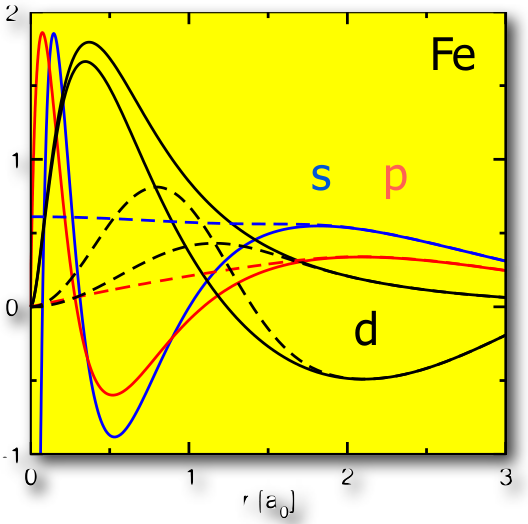
\includegraphics[height=1.2in,width=1.5in,viewport=0 0 570 545,clip]{Figures/PAW-partical.png}
\caption{\small \textrm{The partical-wave of Fe atom.}}%(与文献\cite{EPJB33-47_2003}图1对比)
\label{PAW_partical_Fe}
\end{figure}
}

\frame
{
	\frametitle{\textrm{PAW projector}}
	投影函数:$$|\tilde p_i\rangle=\bigg(-\dfrac12\nabla^2+\tilde v_{at}-\varepsilon_i^1\bigg)|\tilde\phi_i\rangle$$
	\textrm{Gram-Schmidt}正交化
	$$|\tilde p_i\rangle=|\tilde p_i\rangle-\sum_{j=1}^{i-1}|\tilde p_j\rangle\langle\tilde\phi_j|\tilde p_i\rangle$$
%	$$|\phi_i\rangle=|\phi_i\rangle-\sum_{j=1}^{i-1}|\phi_j\rangle\langle\tilde p_j|\tilde\phi_i\rangle$$
%	$$|\tilde\phi_i\rangle=|\tilde\phi_i\rangle-\sum_{j=1}^{i-1}|\tilde\phi_j\rangle\langle\tilde p_j|\tilde\phi_i\rangle$$
	$|\phi_i\rangle=|\phi_i\rangle-\sum\limits_{j=1}^{i-1}|\phi_j\rangle\langle\tilde p_j|\tilde\phi_i\rangle\quad|\tilde\phi_i\rangle=|\tilde\phi_i\rangle-\sum\limits_{j=1}^{i-1}|\tilde\phi_j\rangle\langle\tilde p_j|\tilde\phi_i\rangle$
\begin{figure}[h!]
\centering
\vspace*{-0.4in}
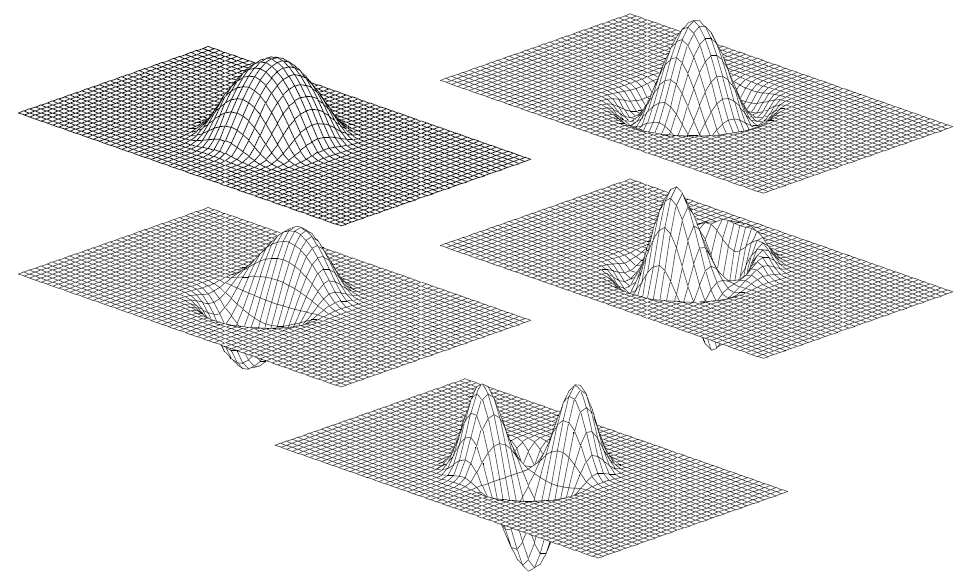
\includegraphics[height=1.5in,width=2.3in,viewport=0 0 1100 745,clip]{Figures/PAW_projector-2.png}
\caption{\small \textrm{The projector of PAW.}}%(与文献\cite{EPJB33-47_2003}图1对比)
\label{PAW_projector}
\end{figure}
\begin{itemize}
	\item 与分波具有相同的角动量$l$
	\item 局域在缀加区域(Augmentation region)
	\item 节点依次增加
\end{itemize}
}

\frame
{
	\frametitle{\textrm{局域势$\bar v$}}
	去屏蔽局域势:$$\bar v(r)=\tilde v_{at}(r)-\int\mathrm{d}r^{\prime}\dfrac{\tilde n(r^{\prime})+\hat n(r^{\prime})}{|r-r^{\prime}|}-\mu_{xc}[\tilde n(r)]$$
	其中$\tilde v_{at}(r)$的确定
	$$\bigg[-\dfrac12\nabla^2+\tilde v_{at}-\varepsilon+\sum_{(i,j)}|\tilde p_i\rangle\big(\mathrm{d}H_{ij}-\varepsilon\mathrm{d}O_{ij}\big)\langle\tilde p_j|\bigg]|\tilde\Psi_j\rangle=0$$
	其中$\mathrm{d}H_{ij}$和$\mathrm{d}O_{ij}$分别是
	$$\mathrm{d}H_{ij}=\langle\phi_i|-\dfrac12\nabla^2+v_{at}|\phi_j\rangle-\langle\tilde\phi_i|-\dfrac12\nabla^2+\tilde v_{at}|\tilde\phi_j\rangle$$
	$$\mathrm{d}O_{ij}=\langle\phi_i|\phi_j\rangle-\langle\tilde\phi_i|\tilde\phi_j\rangle$$
}

\frame
{
	\frametitle{\textrm{局域势$\bar v$}}
	如果解$$|\tilde\Psi\rangle=|u\rangle+\sum_i|w_i\rangle c_i$$
	其中$|u\rangle$和$|w_i\rangle$的定义分别为
	$$\big(-\frac12\nabla^2+\tilde v-\varepsilon\big)|u\rangle=0$$
	$$\big(-\frac12\nabla^2+\tilde v-\varepsilon\big)|w_i\rangle=|\tilde p_i\rangle$$
	因此可以得到
	$$c_i=-\sum_{j,l}\bigg[\delta_{ij}+\sum_k\mathrm{d}H_{ik}-\varepsilon\mathrm{d}O_{ik}\langle\tilde p_k|w_j\rangle\bigg]^{-1}\big(\mathrm{d}H_{jl}-\varepsilon\mathrm{d}O_{jl}\big)\langle p_l|u\rangle$$
}

%\frame
%{
%%	\frametitle{\textrm{PAW}原子数据集}
%	\frametitle{\textrm{PAW Augmentation}}
%\begin{figure}[h!]
%\centering
%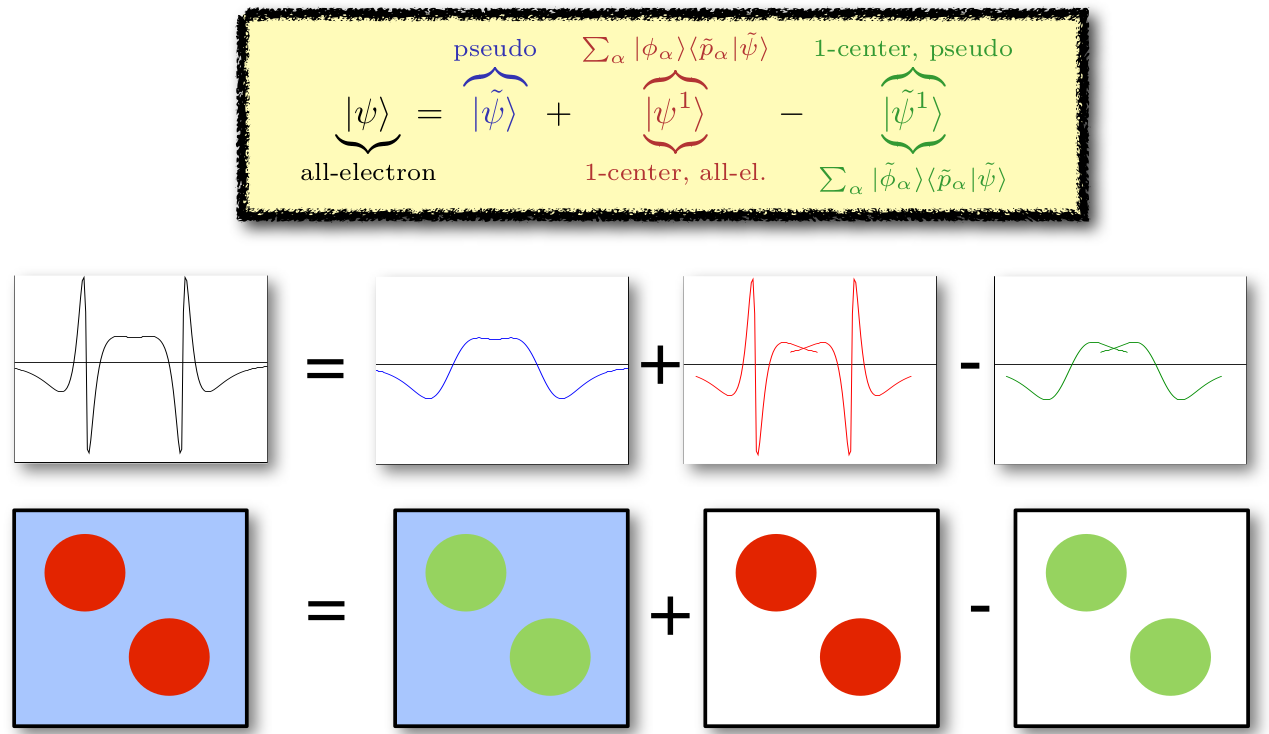
\includegraphics[height=2.3in,width=4.0in,viewport=0 0 1280 745,clip]{Figures/PAW-baseset.png}
%\caption{\small \textrm{The Augmentation of PAW.}}%(与文献\cite{EPJB33-47_2003}图1对比)
%\label{PAW_baiseset}
%\end{figure}
%}

%\frame
%{
%	\frametitle{\textrm{PAW Augmentation}}
%\begin{figure}[h!]
%\centering
%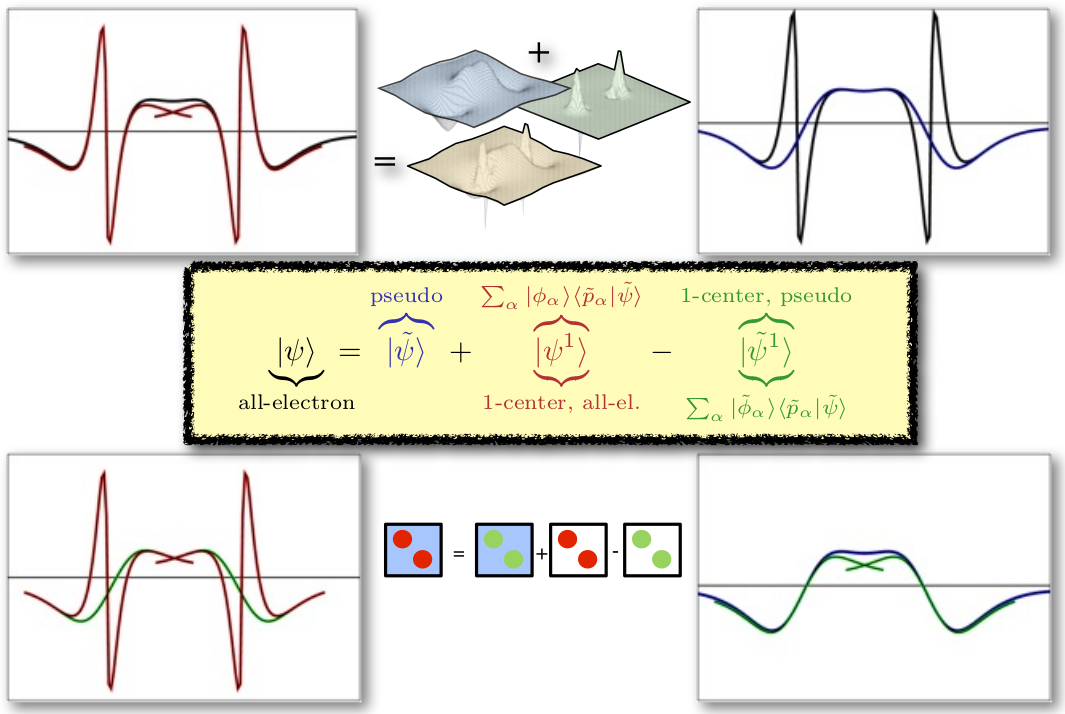
\includegraphics[height=2.3in,width=4.0in,viewport=0 0 1100 745,clip]{Figures/PAW-projector.png}
%\caption{\small \textrm{The projector of PAW.}}%(与文献\cite{EPJB33-47_2003}图1对比)
%\label{PAW_projector}
%\end{figure}
%}

\appendix
\section{基态总能量表达式}
\frame
{
	\frametitle{晶体总能量的一般表示}
采用赝势方法计算的晶体总能量$E_T$由晶格中的电子能量$E_{e-e}$与离子实排斥能$E_{N-N}$之和:
	\begin{displaymath}
		E_T=E_{e-e}+E_{N-N}=T[\rho]+E_{ext}+E_{\mathrm{Coul}}+E_{\mathrm{XC}}+E_{N-N}
	\end{displaymath}
根据\textrm{Kohn-Sham}方程,其中动能泛函用单电子能量表示为
\begin{displaymath}
	T{\rho}=\sum_in_i\langle\psi_i|\varepsilon_i-V_{\mathrm{KS}}|\psi_i\rangle
\end{displaymath}
$n_i$是$\psi_i$上的电子占据数,$\varepsilon_i$是其能量本征值,因此有
\begin{displaymath}
	\hspace*{-12.0pt}	E_T=\sum_in_i\varepsilon_i-\dfrac12\int\int\mathrm{d}\vec r\mathrm{d}\vec r\dfrac{\rho(\vec r)\rho(\vec r^{\prime})}{|\vec r-\vec r^{\prime}|}+\int\mathrm{d}\vec r\rho(\vec r)[\epsilon_{\mathrm{XC}}(\vec r)-V_{\mathrm{XC}}(\vec r)]+E_{N-N}
\end{displaymath}
}

\frame
{
	\frametitle{晶体总能量倒空间的表示}
周期体系的总能量表达式在动量空间($\vec K$空间)计算更方便
\begin{displaymath}
	\hspace*{-18.0pt}	E_T=\sum_in_i\varepsilon_i-\dfrac{\Omega}2\sum_{\vec k\neq 0}\rho^{\ast}(\vec k)V_{\mathrm{Coul}}(\vec k)+\Omega\sum_{\vec k}\rho^{\ast}(\vec k)[\epsilon_{\mathrm{XC}}(\vec k)-V_{\mathrm{XC}}(\vec k)]+E_{N-N}
\end{displaymath}
其中$V_{\mathrm{Coul}}(\vec k)$、$\epsilon_{\mathrm{XC}}(\vec k)$与$\rho^{\ast}(\vec k)$分别是\textrm{Coulomb}相互作用、单个电子的交换-相关能、交换-相关势和电子密度的\textrm{Fourier}分量。

由\textrm{Poisson}方程
\begin{displaymath}
	\nabla^2V_{\mathrm{Coul}}(\vec r)=-4\pi\rho(\vec r)
\end{displaymath}
的\textrm{Fourier}展开有
\begin{displaymath}
	V_{\mathrm{Coul}}(\vec k)=\dfrac{4\pi\rho^{\ast}(\vec k)}{|\vec k|^2}
\end{displaymath}
交换-相关势和交换-相关能的计算一般先在实空间计算$\epsilon_{\mathrm{XC}}(\vec r)$和$V_{\mathrm{XC}}(\vec r)$后,再通过\textrm{Fourier}变换到动量空间,得到$\epsilon_{\mathrm{XC}}(\vec k)$和$V_{\mathrm{XC}}(\vec k)$
}

\frame
{
	\frametitle{晶体离子相互作用的计算}
	离子间\textrm{Coulomb}相互作用能之和
	\begin{displaymath}
		E_{N-N}=\dfrac12\sum_{\vec R,s}\sideset{}{^{\prime}}\sum_{\vec R^{\prime},\vec s^{\prime}}\dfrac{Z_sZ_{s^{\prime}}}{|\vec R+\vec r_s-\vec R^{\prime}-\vec r_s^{\prime}|}
	\end{displaymath}
	这里$Z_s$是离子实的电荷数,$\vec R$表示晶格点的位矢,$\vec r_s$代表元胞内原子的相对位矢。

	\textcolor{red}{\textbf{注意}}:$E_{N-N}$求和包含无穷多项,是发散的;$V_{\mathrm{Coul}}(\vec k=0)$是发散的。
	
	$V_{ext}$在不存在其他外场时,一般只考虑离子-电子的\textrm{Coulomb}相互作用,
	\begin{displaymath}
		\begin{aligned}
			V_{ext}(\vec r)&=\sum_{\vec R,s}\dfrac{-Z_s}{|\vec r-\vec R-\vec r_s|}\\
			&\equiv\sum_{\vec R,s}v_{ext}^s(\vec r-\vec R-\vec r_s)
		\end{aligned}
	\end{displaymath}
}

\frame
{
	\frametitle{晶体总能量计算的奇点排除}
	$V_{ext}$的\textrm{Fourier}分量在$\vec k=0$\textcolor{red}{也是发散的}。这三项单独都是发散的,但因为整个体系出于电中性,所以这些发散项相互抵消,是一个常数。

	因此求解\textrm{Kohn-Sham}方程时,先将$V_{\mathrm{Coul}}(\vec k=0)$和$V_{ext}(\vec k=0)$同时置为零,这相当于\textcolor{red}{将势能作一平移,或者说重新定义势能零点,而在总能量计算中补偿这一平移。}

	发散项之和为:
	\begin{displaymath}
		\begin{aligned}
			\lim_{\vec k\rightarrow0}\Omega&\bigg[\dfrac12V_{\mathrm{Coul}}(\vec k)+\sum_sv_{ext}^s(\vec k)\bigg]\rho^{\ast}(\vec k)+\dfrac12\sum_{\vec R,s}\sideset{}{^{\prime}}\sum_{\vec R^{\prime},\vec s^{\prime}}\dfrac{Z_sZ_{s^{\prime}}}{|\vec R+\vec r_s-\vec R^{\prime}-\vec r_s^{\prime}|}\\
			=&\sum_s\alpha_s\sum_sZ_s+E_{\mathrm{Ewald}}
		\end{aligned}
	\end{displaymath}
}

\frame
{
	\frametitle{发散项的处理}
	对于形如$Z_s/r$的外场,其\textrm{Fourier}分量在$\vec k=0$附近展开
	\begin{displaymath}
		v_{ext}^s(\vec k)=-\dfrac{4\pi Z_s}{\Omega|\vec k|^2}+\alpha_s+O(\vec k); 
	\end{displaymath}
	展开$\rho^{\ast}(\vec k)$,有
	\begin{displaymath}
		\lim_{\vec k\rightarrow 0}\rho^{\ast}(\vec k)=\dfrac{\sum_sZ_s}{\Omega}+\beta|\vec k|^2+O(\vec k)
	\end{displaymath}
去掉高次项,有
\begin{displaymath}
	\begin{aligned}
		\lim_{\vec k\rightarrow 0}&\bigg[\dfrac{\Omega}2\dfrac{4\pi[\rho^{\ast}(\vec k)]^2}{|\vec k|^2}+\Omega\bigg(-\dfrac{4\pi\sum_sZ_s}{\Omega|\vec k|^2}+\sum_s\alpha_s\bigg)\rho^{\ast}(\vec k)+\dfrac12\dfrac{8\pi(\sum_sZ_s)^2}{\Omega|\vec k|^2}\bigg]\\
		&+\dfrac12\sum_{\vec R,s}\sideset{}{^{\prime}}\sum_{\vec R^{\prime},\vec s^{\prime}}\dfrac{Z_sZ_{s^{\prime}}}{|\vec R+\vec r_s-\vec R^{\prime}-\vec r_{s^{\prime}}|}-\lim_{\vec k\rightarrow0}\dfrac12\dfrac{4\pi(\sum_sZ_s)^2}{\Omega|\vec k|^2}\\
		=&\sum_s\alpha_s\sum_sZ_s+E_{\mathrm{Ewald}}
	\end{aligned}
\end{displaymath}
}

\frame
{
	\frametitle{离子间相互作用的\textrm{Ewald}求和}
	\begin{displaymath}
		\begin{aligned}
			E_{\textrm{Ewald}}=&\dfrac12\sum_{\vec R,s}\sideset{}{^{\prime}}\sum_{\vec R^{\prime},\vec s^{\prime}}\dfrac{Z_sZ_{s^{\prime}}}{|\vec R+\vec r_s-\vec R^{\prime}-\vec r_{s^{\prime}}|}-\lim_{\vec k\rightarrow0}\dfrac12\times\dfrac{4\pi(\sum_sZ_s)^2}{\Omega|\vec k|^2}\\
			=&\dfrac12\sum_{\vec R,s}\sideset{}{^{\prime}}\sum_{\vec R^{\prime},\vec s^{\prime}}\dfrac{Z_sZ_{s^{\prime}}}{|\vec R+\vec r_s-\vec R^{\prime}-\vec r_{s^{\prime}}|}-\dfrac1{2\Omega}\sum_{s,s^{\prime}}\int\mathrm{d}\vec r\dfrac{Z_sZ_{s^{\prime}}}r\\
			=&\sum_{s,s^{\prime}}Z_sZ_{s^{\prime}}\bigg\{\dfrac{2\pi}{\Omega}\sum_{\vec k\neq 0}\cos[\vec k\cdot(\vec r_s-\vec r_{s^{\prime}})]\dfrac{\mathrm{e}^{-|\vec k|^2/4\eta^2}}{|\vec k|^2}\\
			&-\dfrac{\pi}{2\eta^2\Omega}+\dfrac14\sum_{\vec R}\dfrac{\mathrm{erf}(\eta x)}x\bigg|_{\vec R+\vec r_s-\vec r_s^{\prime}\neq0}-\dfrac{\eta}{\sqrt{\pi}}\delta_{s,s^{\prime}}\bigg\}
		\end{aligned}
	\end{displaymath}
	$\mathrm{erf}(x)$是误差函数,$\eta$原则上是任意参数。$\alpha_s$由$v_{ext}^s(\vec r)$确定:
	\begin{displaymath}
		\alpha_s=\lim_{\vec k\rightarrow0}\bigg[v_{ext}^s(\vec k)+\dfrac{4\pi Z_s}{\Omega|\vec k|^2}\bigg]=\dfrac1{\Omega}\int\mathrm{d}\vec r\bigg[v_{ext}^s(\vec r)+\dfrac{Z_s}r\bigg]
	\end{displaymath}
}

\frame
{
	\frametitle{总能量表达式}
由此得到的总能量表达式是
\begin{displaymath}
	\begin{aligned}
		E_T=&\sum_i\varepsilon_i-\dfrac{\Omega}2\sum_{\vec k\neq0}\rho^{\ast}(\vec k)V_{\mathrm{Coul}}(\vec k)\\
		&+\Omega\sum_{\vec k}\rho^{\ast}(\vec k)[\epsilon_{\mathrm{XC}}(\vec k)-V_{\mathrm{XC}}(\vec k)]\\
		&+\sum_s\alpha_s\sum_sZ_s+E_{\mathrm{Ewald}}
	\end{aligned}
\end{displaymath}
}

%------------------------------------------------------------------------Reference----------------------------------------------------------------------------------------------
%\begin{thebibliography}{99}
%-----------------------------------------------------------------------------------------------------------------------------------------------------------------------%
%\frame
%{
%\frametitle{主要参考文献}
%{\small
%\bibitem{Singh_Book}\textrm{D. J. Singh. \textit{Plane Wave, PseudoPotential and the LAPW method} (Kluwer Academic, Boston,USA, 1994)}					%
%  \nocite{*}																				%
%}
%}
%\end{thebibliography}
\begin{thebibliography}{99}
\frame
{
\frametitle{主要参考文献}
{\small
%	\bibitem{Huang_Han}黄昆\:原著、韩汝琦\:改编, {\textit{固体物理学}}\:高等教育出版社, 北京, 1988
	\bibitem{Xie_Lu}谢希德、陆栋\:主编, {\textit{固体能带理论}}\:复旦大学出版社, 上海, 1998
	\bibitem{Elect_Stru}\textrm{Richard. M. Martin. \textit{Electronic Structure: Basic Theory and Practical Methods} (Cambridge University Press, Cambridge, England, 2004)}
        \bibitem{Singh_Book}\textrm{D. J. Singh. \textit{Plane Wave, PseudoPotential and the LAPW method} (Kluwer Academic, Boston,USA, 1994)}
        \bibitem{JPCM6-8245_1994}\textrm{G. Kresse and J. Hafner. J. Phys: \textit{Condens. Matter}, \textbf{6} (1994), 8245}
        \bibitem{PRB50-17953_1994}\textrm{P. E. Bl\"ochl. \textit{Phys. Rev.} B, \textbf{50} (1994), 17953}
}
\nocite*{}
}
\end{thebibliography}
%{\small
%\phantomsection\addcontentsline{toc}{section}{Bibliography}	 %直接调用\addcontentsline命令可能导致超链指向不准确,一般需要在之前调用一次\phantomsection命令加以修正	%
%\bibliography{Myref}																			%
%\bibliographystyle{mybib}																		%
%  \nocite{*}																				%
%}
%-----------------------------------------------------------------------------------------------------------------------------------------------------------------------%


%-----------------------------------------------------------Beamer下不建议使用bib,因为涉及分页--------------------------------------------------------------------------%
%{\small
%\phantomsection\addcontentsline{toc}{section}{Bibliography}	 %直接调用\addcontentsline命令可能导致超链指向不准确,一般需要在之前调用一次\phantomsection命令加以修正	%
%\bibliography{Myref}																			%
%\bibliographystyle{mybib}																		%
%  \nocite{*}																				%
%}

%------------------------------------------------------------------------------------------------------------------------------------------------------------------------------%

%-------------------------------------------------------------------------Thanks------------------------------------------------------------------------------------------------
%\section{致谢}
%\frame
%{
%\frametitle{致$\quad$谢}
%\begin{itemize}
%    \setlength{\itemsep}{20pt}
%  \item 感谢本团队高兴誉、吴泉生、宋红州等各位老师参与的讨论
%  \item 感谢莫所长、宋主任以及软件中心各位老师和同事
%  \item 感谢王崇愚先生的帮助
%\end{itemize}
%}
\frame
{
\vskip 60 pt
%\hskip 10pt \textcolor{blue}{\Huge 感谢答辩委员会各位老师\,\textrm{!}}\\
\vskip 35 pt
\hskip 60pt \textcolor{blue}{\Huge 谢谢大家\:!}
%\vskip 15 pt
%\hskip 40pt \textcolor{blue}{\Huge \textrm{for your attention\:!}}
}

%-------------------------------------------------------------------------------------------------------------------------------------------------------------------------------

\clearpage
%\end{CJK*}
\end{document}
